\documentclass{beamer}

\usepackage[utf8x]{inputenc}
\usepackage{default}
\usepackage{graphicx}

\begin{document}

\begin{frame}
Cluster de ganeti:\\
 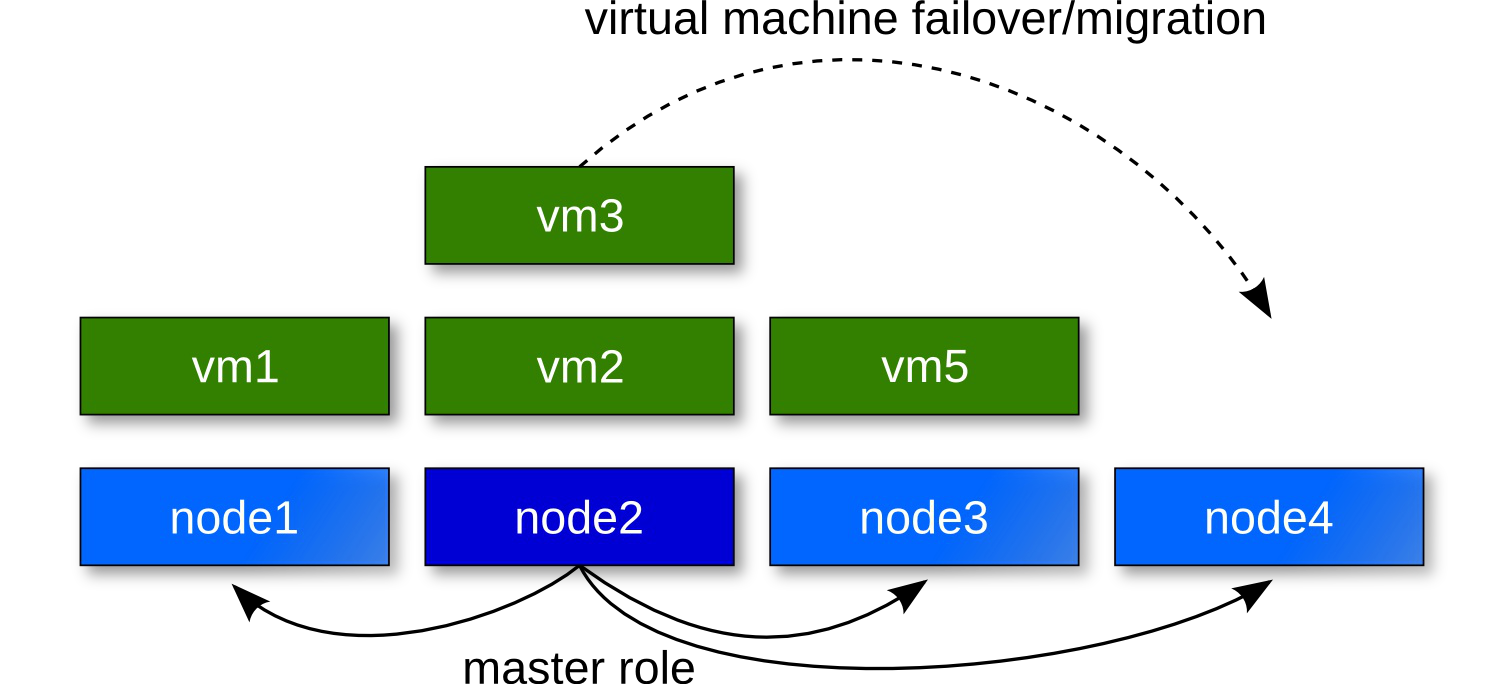
\includegraphics[width=10cm,height=5cm]{images/ganeti_cluster.png}
\end{frame}

\begin{frame}
Ganeti, qu'est-ce que c'est?\\
\begin{itemize}
\item Un outil de gestion de cluster de serveur virtuel
\item Il utilise l'hyperviseurs existant (XEN hypervisor,kvm)
\item Récupération rapide et simple, après des crashs physique
\item Utilisation de peu de ressources matériel
\item IaaS privés (L'infrastructure en tant que service)
\end{itemize}
\end{frame}

\begin{frame}
Background du projet:\\
\begin{itemize}
\item Projet financé par Google
\item Open source depuis 2007 GPLv2
\item Équipe Google basée en Suisse
\item Liste de diffusion active et canal IRC
\end{itemize}
Organisations utilisant ganeti:\\
\begin{itemize}
\item Google (utilisé dans leur infrastructure)
\item Ggrnet.gr (Greek Research \& Technology Network)
\item osuosl.org (Oregon State University Open Source Lab)
\end{itemize}
\end{frame}

\begin{frame}
Composants:\\
\begin{itemize}
\item Python et quelques modules
\item Haskell
\item DRBD
\item LVM
\item Hyperviseur
\end{itemize}

\includegraphics[width=7cm,height=1.5cm]{images/module.png}
\end{frame}

\begin{frame}
Architechture:\\
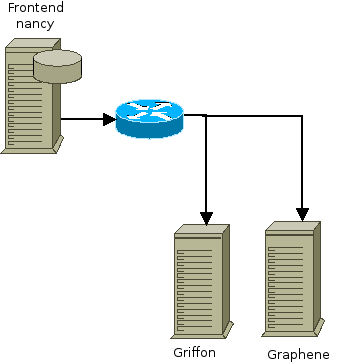
\includegraphics[width=8cm,height=4cm]{images/archi.png}
\end{frame}

\begin{frame}
Noeud:\\
\begin{itemize}
\item machine physique
\item La tolérance aux pannes n'est pas nécessaire
\item Ajouté / supprimé à volonté à partir du cluster
\item Aucune perte de données avec une perte de noeud
\end{itemize}
\end{frame}

\begin{frame}
Daemons:\\
\begin{itemize}
\item ganeti-noded : contrôler les ressources matérielles, qui fonctionne sur tous les noeuds
\item ganeti-confd : seulement fonctionnel sur le maître, et s'exécute sur tous les noeuds
\item ganeti-rapi : seulement sur l'API-HTTP  pour le cluster, fonctionne sur le maître
\item ganeti-masterd :  permet un contrôle du cluster, fonctionne sur le maître
\end{itemize}
\end{frame}

\begin{frame}
Instance:\\
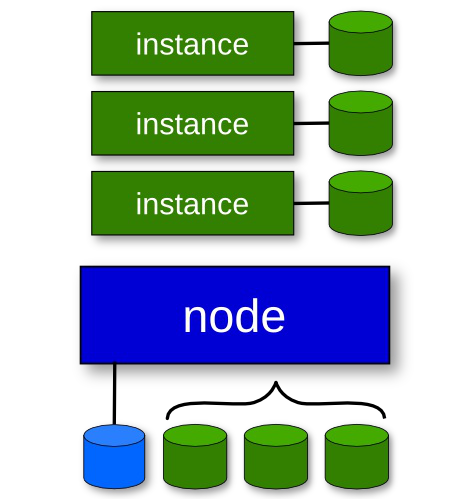
\includegraphics[width=3cm,height=3cm]{images/instance.png}
\begin{itemize}
\item Machine virtuelle qui s'exécute sur le cluster
\item tolérant aux pannes / Haute disponibilité au sein du cluster
\end{itemize}
\end{frame}

\begin{frame}
Distributions suportées:\\
\begin{itemize}
\item Debian - trés bien supporté
\item Gentoo - un support est apporté pour l'installation
\item Ubuntu - devrait fonctionner
\item CentOS - fonctionne mais quelques problèmes d'installation
\end{itemize}
\end{frame}

\begin{frame}
planification réseau:\\

\includegraphics[width=3cm,height=3cm]{images/network.png}
\begin{itemize}
\item La connexion via un bridge est la supportée
\item Un réseau routé est également soutenu
\item Noeuds sur un NAT privé
\end{itemize}
\end{frame}

\begin{frame}
configuration du système d'exploitation:\\
\begin{itemize}
\item installation minimale du système
\item Minimum le volume du système de 20 Go
\item Simple groupe de volumes LVM pour les instances
\item 64bit est préférable
\item Matériel / logiciels similaires pour la configuration des nœuds
\end{itemize}
\end{frame}

\begin{frame}
Hyperviseur requis:\\
Obligatoire sur tous les nœuds
\begin{itemize}
\item Xen 3.0 et au-dessus \\ou
\item KVM 0,11 et au-dessus
\end{itemize}
\end{frame}

\begin{frame}
Installation:\\
\begin{itemize}
\item Installation (facile par les dépots) et configuration de ganeti pour le réseau
\item Pour la haute disponibilité il faut installer et configurer DRDB pour le réseau
\end{itemize}
\end{frame}

\begin{frame}
Ce qui est installé:\\
\begin{itemize}
\item Bibliothèques Python sous le nom ganeti
\item Ensemble des programmes dans / usr / local / sbin ou / usr / sbin
\item Ensemble d'outils dans lib / ganeti / répertoire des outils
\item Scripts IAllocator sous lib / ganeti / outils annuaire
\item Cron jobs nécessaires pour la maintenance du cluster
\item Script d'initialisation pour les démons ganeti
\end{itemize}
\end{frame}


\end{document}
